In what follows, we use the notation $(x_1,y_1)$ to represent a point in
the $(x,y)$ coordinate system, also called the $(x,y)$-plane.
Previously, we used $(a,b)$ to represent
an open interval. Notation often gets reused and abused in mathematics, 
but thankfully, it is usually clear from the context what we mean.

In the $(x,y)$ coordinate system we normally write the $x$-axis
horizontally, with positive numbers to the right of the origin, and
the $y$-axis vertically, with positive numbers above the origin.  That
is, unless stated otherwise, we take ``rightward'' to be the positive
$x$-direction and ``upward'' to be the positive $y$-direction.  In a
purely mathematical situation, we normally choose the same scale for
the $x$- and $y$-axes.  For example, the line joining the origin to
the point $(a,a)$ makes an angle of 45${}^\circ$ with the $x$-axis
(and also with the $y$-axis).

In applications, often letters other than $x$ and $y$ are used, and
often different scales are chosen in the horizontal and vertical
directions.  \\

\begin{example}{Data Plot}{DataPlot}
Suppose you drop a coin from a window, and you want to study how 
its height above the ground changes from second to second.
It is natural to let the letter $t$ denote the time
(the number of seconds since the object was released) and to let the
letter $h$ denote the height.  For each $t$ (say, at one-second
intervals) you have a corresponding height $h$.  This information can
be tabulated, and then plotted on the $(t,h)$ coordinate plane, as
shown in figure~\ref{fig:data plot}.
\end{example}

\figure[!ht]
\vbox{
$$\begin{array}{|r|ccccc|}
\hline
seconds & 0 & 1 & 2 & 3 & 4\\
\hline
meters & 80 & 75.1 & 60.4 & 35.9 & 1.6\\
\hline
\end{array}$$ 

\centerline{\vbox{\beginpicture
\normalgraphs
%\ninepoint
\setcoordinatesystem units <2truecm,0.5truemm>
\setplotarea x from 0 to 4.2, y from 0 to 90
\axis left shiftedto x=0 ticks numbered from 20 to 80 by 20 /
\axis bottom shiftedto y=0 ticks numbered from 0 to 4 by 1 /
\put {$t$} [l] <3pt,0pt> at 4.2 0
\put {$h$} [l] <3pt,0pt> at 0 90
\setquadratic
\plot 0 80 1 75.1 2 60.4 3 35.9 4 1.6 /
\multiput {$\bullet$} at 0 80 1 75.1 2 60.4 3 35.9 4 1.6 /
\endpicture}}}
\caption{A data plot, height versus time. \label{fig:data plot}}
\endfigure

We use the word ``quadrant'' for each of the four regions into which
the plane is divided by the axes: the first quadrant is where points
have both coordinates positive, or the ``northeast'' portion of the
plot, and the second, third, and fourth quadrants are counted off
counterclockwise, so the second quadrant is the northwest, the third
is the southwest, and the fourth is the southeast.

Suppose we have two points $A$ and $B$ in the $(x,y)$-plane.
We often want to know the change in $x$-coordinate (also called the
``horizontal distance'') in going from $A$ to $B$.  This is often
written $\Delta x$, where the meaning of $\Delta$ (a capital delta in
the Greek alphabet) is ``change in''. Thus, $\Delta x$ can be read as
``change in $x$'' although it usually is read as ``delta $x$''. The
point is that $\Delta x$ denotes a single number, and should not be
interpreted as ``delta times $x$''. Similarly, the ``change in $y$'' is written $\Delta y$
and represents the difference between the $y$-coordinates of the 
two points. It is the vertical distance you have to move in going from $A$ to $B$. \\

\begin{example}{Change in $x$ and $y$}{ChangeIn}\label{ChangeIn}
If $A=(2,1)$ and $B=(3,3)$ the change in $x$ is
$$\Delta x=3-2=1$$
while the change in $y$ is
$$\Delta y= 3-1=2.$$
\vspace{-0.5cm}
\end{example}

The general formulas for the change in $x$ and the change in $y$ 
between a point $(x_1,y_1)$ and a point $(x_2,y_2)$ are:
$$
\Delta x=x_2-x_1,\qquad\qquad\Delta y=y_2-y_1.
$$
Note that either or both of these might be negative.



%%%%%%%%%%%%%%%%%%
\subsection{Lines}
If we have two \ifont{distinct} points $A(x_1,y_1)$ and $B(x_2,y_2)$, then we can draw one
and only one straight line through both points.  By the \dfont{slope} of this line
we mean the ratio of $\Delta y$ to $\Delta x$.  The slope is often denoted by the letter $m$. \\

\begin{formulabox}[Slope Formula]
The slope of the line joining the points $(x_1,y_1)$ and $(x_2,y_2)$ is:
$$m=\frac{\Delta y}{\Delta x}=\frac{(y_2-y_1)}{(x_2-x_1)}=\frac{\mbox{rise}}{\mbox{run}}.$$
\end{formulabox}

\bigskip

\begin{example}{Slope of a Line Joining Two Points}{SlopeofLine}
The line joining the two points $(1,-2)$ and $(3,5)$ has slope
$\ds m=\frac{5-(-2)}{3-1}=\frac{7}{2}$.
%\vspace{-0.8cm}
\end{example}

The most familiar form of the equation of a straight line is:
$$y=mx+b.$$
Here $m$ is the slope of the line: if you increase $x$ by
1, the equation tells you that you have to increase $y$ by $m$; and if
you increase $x$ by $\Delta x$, then $y$ increases by $\Delta
y=m\Delta x$.  The number $b$ is called the \dfont{y-intercept}, because
it is where the line crosses the $y$-axis (when $x=0$).  If you know two points on
a line, the formula $m=(y_2-y_1)/(x_2-x_1)$ gives you the slope.
Once you know a point and the slope, then the $y$-intercept can be
found by substituting the coordinates of either point in the equation:
$y_1=mx_1+b$, i.e., $b=y_1-mx_1$.  Alternatively, one can use the
\dfont{``point-slope'' form} of the equation of a straight line: start with
$(y-y_1)/(x-x_1)=m$ and then multiply to get 
$$(y-y_1)=m(x-x_1),$$ the
point-slope form. Of course, this may be further manipulated to get
$y=mx-mx_1+y_1$, which is essentially the \dfont{``$y=mx+b$'' form}.

It is possible to find the equation of a line between two points directly
from the relation $m=(y-y_1)/(x-x_1)=(y_2-y_1)/(x_2-x_1)$, which says ``the
slope measured between the point $(x_1,y_1)$ and the point $(x_2,y_2)$ is
the same as the slope measured between the point $(x_1,y_1)$ and any other
point $(x,y)$ on the line.''  For example, if we want to find the equation
of the line joining our earlier points $A(2,1)$ and $B(3,3)$, we can use
this formula:
$$
m=\frac{y-1}{x-2}=\frac{3-1}{3-2}=2,\qquad\hbox{so~that}\qquad
y-1=2(x-2),\qquad\hbox{i.e.,}\qquad y=2x-3.
$$
Of course, this is really just the point-slope formula, except that we
are not computing $m$ in a separate step. 
We summarize the three common forms of writing a straight line below:\\

\begin{formulabox}[Slope-Intercept Form of a Straight Line]
An equation of a line with slope $m$ and $y$-intercept $b$ is:
$$y=mx+b.$$
\end{formulabox}

\bigskip

\begin{formulabox}[Point-Slope Form of a Straight Line]
An equation of a line passing through $(x_1,y_1)$ and having slope $m$ is:
$$y-y_1=m(x-x_1).$$
\end{formulabox}

\bigskip

\begin{formulabox}[General Form of a Straight Line]
Any line can be written in the form
$$Ax+By+C=0,$$
where $A,B,C$ are constants and $A,B$ are not both $0$.
\end{formulabox}

The slope $m$ of a line in the form $y=mx+b$ tells us the
direction in which the line is pointing.  If $m$ is positive, the line goes
into the 1st quadrant as you go from left to right.   If $m$ is large and
positive, it has a steep incline, while if $m$ is small and positive, 
then the line has a small angle of inclination.  If $m$ is negative, the
line goes into the 4th quadrant as you go from left to right.  If $m$ is
a large negative number (large in absolute value), then the line points
steeply downward. If $m$ is negative but small in absolute value, then it points
only a little downward.

If $m=0$, then the line is horizontal and its equation is simply $y=b$.

All of these possibilities are illustrated below.
%figure~\ref{fig:graphs of lines}.

$$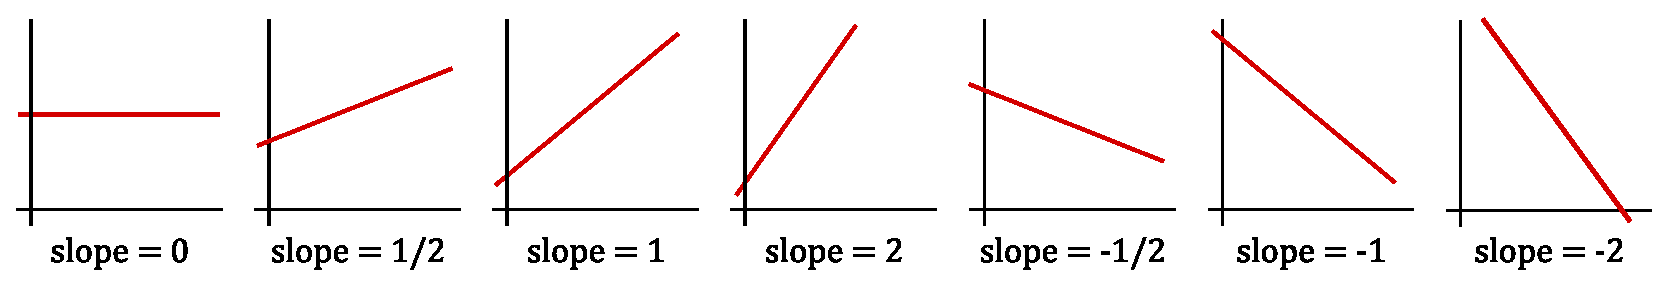
\includegraphics[width=6.4in]{images/slopes}$$

%\figure[!ht]
%\vbox{
%\centerline{\vbox{\beginpicture
%\normalgraphs
%%\sevenpoint
%\setcoordinatesystem units <3truemm,3truemm>
%\setplotarea x from -5 to 5, y from -5 to 5
%\axis left shiftedto x=0 /
%\axis bottom shiftedto y=0 /
%\setlinear
%\plot -1 -5 2.33 5 /
%\linethickness 0.1pt
%\axis left ticks in andacross from -5 to 5 by 1 /
%\axis left ticks in andacross numbered from -4 to 4 by 2 /
%\axis bottom ticks in andacross from -5 to 5 by 1 /
%\axis bottom ticks in andacross numbered from -4 to 4 by 2 /
%\endpicture}\qquad\vbox{\beginpicture
%\normalgraphs
%%\sevenpoint
%\setcoordinatesystem units <3truemm,3truemm>
%\setplotarea x from -5 to 5, y from -5 to 5
%\axis left shiftedto x=0 /
%\axis bottom shiftedto y=0 /
%\setlinear
%\plot -5 1 5 2 /
%\linethickness 0.1pt
%\axis left ticks in andacross from -5 to 5 by 1 /
%\axis left ticks in andacross numbered from -4 to 4 by 2 /
%\axis bottom ticks in andacross from -5 to 5 by 1 /
%\axis bottom ticks in andacross numbered from -4 to 4 by 2 /
%\endpicture}\qquad\vbox{\beginpicture
%\normalgraphs
%%\sevenpoint
%\setcoordinatesystem units <3truemm,3truemm>
%\setplotarea x from -5 to 5, y from -5 to 5
%\axis left shiftedto x=0 /
%\axis bottom shiftedto y=0 /
%\setlinear
%\plot -0.5 5 2 -5 /
%\linethickness 0.1pt
%\axis left ticks in andacross from -5 to 5 by 1 /
%\axis left ticks in andacross numbered from -4 to 4 by 2 /
%\axis bottom ticks in andacross from -5 to 5 by 1 /
%\axis bottom ticks in andacross numbered from -4 to 4 by 2 /
%\endpicture}\qquad\vbox{\beginpicture
%\normalgraphs
%%\sevenpoint
%\setcoordinatesystem units <3truemm,3truemm>
%\setplotarea x from -5 to 5, y from -5 to 5
%\axis left shiftedto x=0 /
%\axis bottom shiftedto y=0 /
%\setlinear
%\plot -5 2 5 1 /
%\linethickness 0.1pt
%\axis left ticks in andacross from -5 to 5 by 1 /
%\axis left ticks in andacross numbered from -4 to 4 by 2 /
%\axis bottom ticks in andacross from -5 to 5 by 1 /
%\axis bottom ticks in andacross numbered from -4 to 4 by 2 /
%\endpicture}}}
%\caption{Lines with slopes 3, $0.1$, $-4$, and $-0.1$.\label{fig:graphs of lines}}
%\endfigure

There is one type of line that cannot be written in the form $y=mx+b$,
namely, vertical lines.  A vertical line has an equation of the form $x=a$.
Sometimes one says that a vertical line has an ``infinite'' slope.

It is often useful to find the $x$-intercept of a line $y=mx+b$.  This is
the $x$-value when $y=0$.  Setting $mx+b$ equal to 0 and solving for
$x$ gives: $x=-b/m$.  \\

\begin{example}{Finding $x$-intercepts}{xintercepts}
To find $x$-intercept(s) of the line $y=2x-3$ we set $y=0$ and solve for $x$:
$$0 = 2x-3\qquad\to\qquad x = \frac{3}{2}.$$
Thus, the line has an $x$-intercept of $3/2$.
\end{example}

It is often necessary to know if two lines are parallel or perpendicular.
Let $m_1$ and $m_2$ be the slopes of the nonvertical lines $L_1$ and $L_2$.
Then:
\begin{itemize}
\item $L_1$ and $L_2$ are \dfont{parallel} if and only if $m_1=m_2$.
\item $L_1$ and $L_2$ are \dfont{perpendicular} if and only if $\ds{m_2=\frac{-1}{m_1}}$.
\end{itemize}
In the case of perpendicular lines, we say their slopes are \ifont{negative reciprocals}. 
Below is a visual representation of a pair of parallel lines and a pair of perpendicular lines.
$$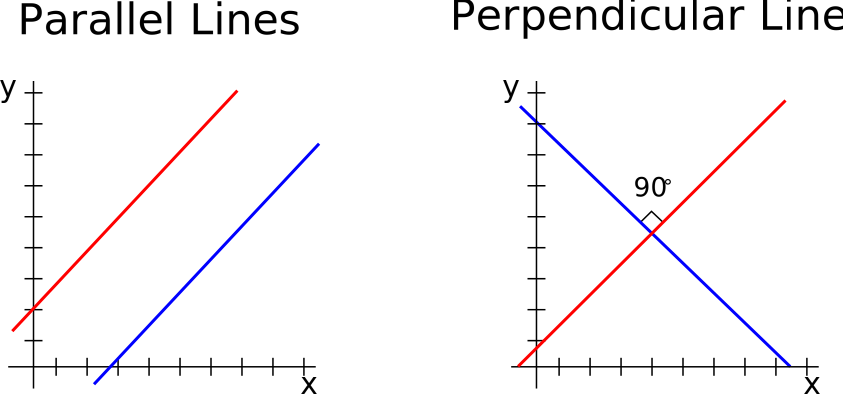
\includegraphics[width=3.7in]{images/lines-1}$$

\begin{example}{Equation of a Line}{EquationLine}
For each part below, find an equation of a line satisfying the requirements:
\begin{enumerate}
\item[(a)] Through the two points $(0,3)$ and $(-2,4)$.
\item[(b)] With slope $7$ and through point $(1,-2)$.
\item[(c)] With slope $2$ and $y$-intercept $4$.
\item[(d)] With $x$-intercept $8$ and $y$-intercept $-3$.
\item[(e)] Through point $(5,3)$ and parallel to the line $2x+4y+2=0$.
\item[(f)] With $y$-intercept $4$ and perpendicular to the line $\ds{y=-\frac{2}{3}x+3}$.
\end{enumerate}
\end{example}

\begin{solution} 
\noindent(a) We use the \ifont{slope formula} on $(x_1,y_1)=(0,3)$ and $(x_2,y_2)=(-2,4)$ to find m:
$$m=\frac{(4)-(3)}{(-2)-(0)}=\frac{1}{-2}=-\frac{1}{2}.$$
Now using the \ifont{point-slope formula} we get an equation to be:
$$y-3=-\frac{1}{2}\left(x-0\right)\quad\to\quad y=-\frac{1}{2}x+3.$$

\noindent(b) Using the \ifont{point-slope formula} with $m=7$ and $(x_1,y_1)=(1,-2)$ gives:
$$y-(-2)=7(x-1)\quad\to\quad y = 7x-9.$$

\noindent(c) Using the \ifont{slope-intercept formula} with $m=2$ and $b=4$ we get $y=2x+4$.

\noindent(d) Note that the intercepts give us two points: $(x_1,y_1)=(8,0)$ and $(x_2,y_2)=(0,-3)$.
Now follow the steps in part (a):
$$m=\frac{-3-0}{0-8}=\frac{3}{8}$$.
Using the \ifont{point-slope formula} we get an equation to be:
$$y-(-3)=\frac{3}{8}\left(x-0\right)\quad\to\quad y=\frac{3}{8}x-3$$.

\noindent(e)  The line $2x+4y+2=0$ can be written as:
$$4y = -2x - 2 \quad\to\quad y=-\frac{1}{2}x-\frac{1}{2}.$$
This line has slope $-1/2$.
Since our line is \ifont{parallel} to it, we have $m=-1/2$.
Now we have a point $(x_1,y_1)=(5,3)$ and slope $m=-1/2$, thus, the \ifont{point-slope formula} gives:
$$y-3=-\frac{1}{2}\left(x-5\right).$$

\noindent(f) The line $\ds{y=-\frac{2}{3}x+3}$ has slope $m=-2/3$.
Since our line is perpendicular to it, the slope of our line is the \ifont{negative reciprocal}, hence, $m=3/2$.
Now we have $b=4$ and $m=3/2$, thus by the \ifont{slope-intercept formula}, an equation of the line is
$$y=\frac{3}{2}x+4.$$
\vspace{-0.5cm}
\end{solution}

\bigskip
\begin{example}{Parallel and Perpendicular Lines}{ParallelPerpendicularLines}
Are the two lines $7x+2y+3=0$ and $6x-4y+2=0$ perpendicular? Are they parallel? If they are not parallel, what is their point of intersection?
\end{example}

\begin{solution} 
The first line is:
$$7x+2y+3=0\quad\to\quad 2y=-7x-3\quad\to\quad y=-\frac{7}{2}x-\frac{3}{2}.$$
It has slope $m_1=-7/2$.
The second line is:
$$6x-4y+2=0\quad\to\quad -4y=-6x-2\quad\to\quad y=\frac{3}{2}x+\frac{1}{2}.$$
It has slope $m_2=3/2$.
Since $m_1\cdot m_2\neq -1$ (they are not negative reciprocals), the lines are not perpendicular.
Since $m_1\neq m_2$ the lines are not parallel.

We find points of intersection by setting $y$-values to be the same and solving.
In particular, we have
$$-\frac{7}{2}x-\frac{3}{2}=\frac{3}{2}x+\frac{1}{2}.$$
Solving for $x$ gives $x=-2/5$. Then substituting this into either equation gives $y=-1/10$.
Therefore, the lines intersect at the point $(-2/5,-1/10)$.
\end{solution}


